% The contents of this file is 
% Copyright (c) 2009-  Charles R. Severance, All Righs Reserved

\chapter{Timeline of Computer Science}\label{appendixTimeline}

The timeline on the following pages depicts some milestones from CS's long history. It is based on a curated list from Scott Aaronson\footnote{Taken from Shtetl-Optimized: The Blog of Scott Aaronson; \url{https://www.scottaaronson.com/blog/?p=524}}. With its intention to collapse thousands of years of events into a few pages, the timeline is interesting but necessarily incomplete. Note that the timeline ends in 2011. Exercise \ref{exCh18Timeline} on page \pageref{exCh18Timeline} asks you to bring it up to date.

\begin{figure}[H]
	\begin{center}
		\caption{Beginning through 1799}
		\vskip 4pt
		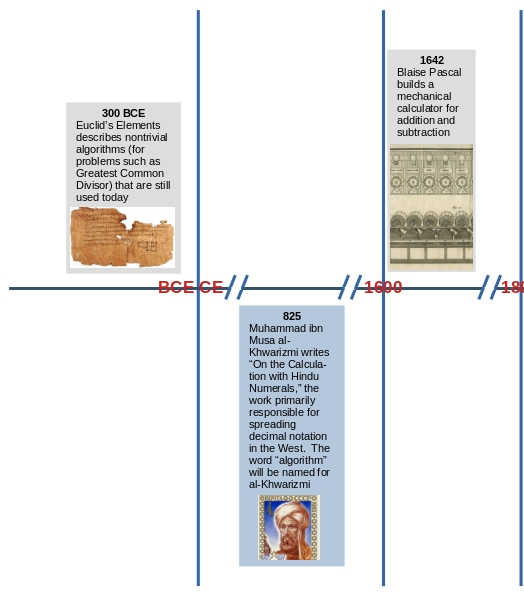
\includegraphics[height=5.5in]{cs-timeline/CSHistoryTimeline-Part1a.jpg}
	\end{center}
\end{figure}

\begin{figure}[H]
	\begin{center}
		\caption{1800 through 1949}
		\vskip 4pt
		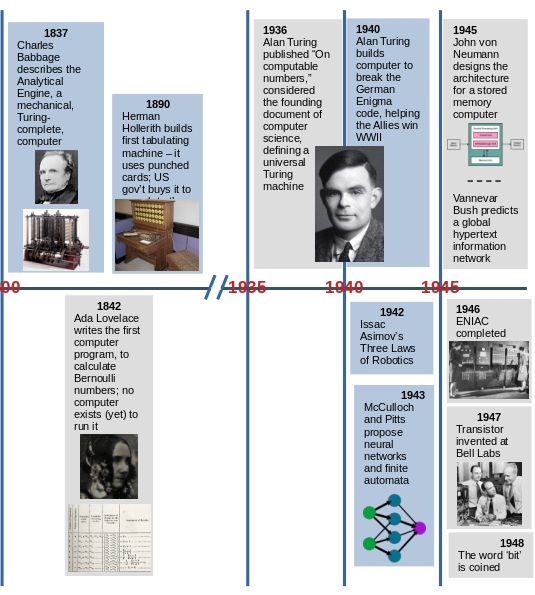
\includegraphics[height=5.5in]{cs-timeline/CSHistoryTimeline-Part1b.jpg}
	\end{center}
\end{figure}

\begin{figure}[H]
	\begin{center}
		\caption{1950 through 1979}
		\vskip 4pt
		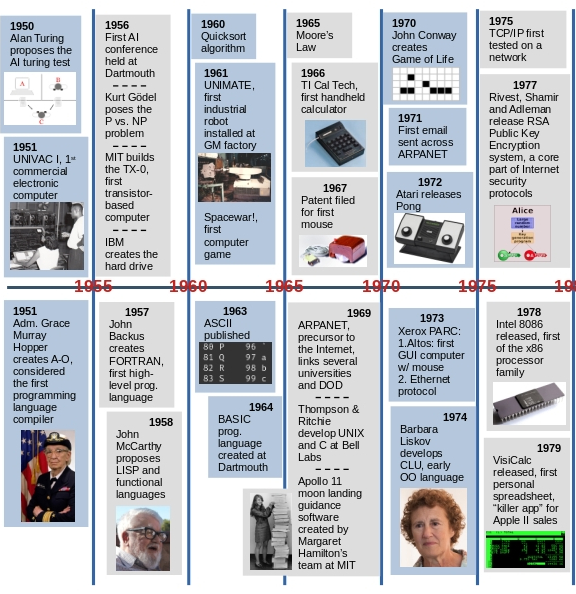
\includegraphics[height=5in]{cs-timeline/CSHistoryTimeline-Part2a.jpg}
	\end{center}
\end{figure}

\begin{figure}[H]
	\begin{center}
		\caption{1980 through 2011}
		\vskip 4pt
		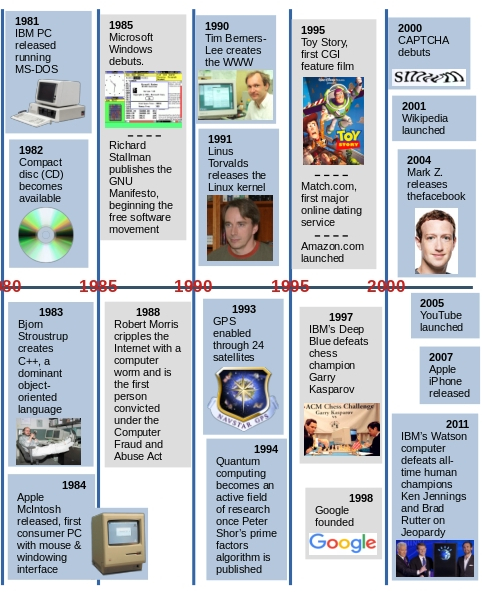
\includegraphics[height=5.5in]{cs-timeline/CSHistoryTimeline-Part2b.jpg}
	\end{center}
\end{figure}

\newpage

\section{Image sources}

\begin{longtable}[H]{p{.4in}|p{.8in}|p{3in}}
	\caption{Image Sources}\\
	\textbf{Year} & textbf{Item} & \textbf{Source}\\
	\hline
	\endfirsthead
	\textbf{Year} & textbf{Item} & \textbf{Source}\\
	\endhead
	\Tstrut 300 & Euclid's Elements & https://en.wikipedia.org/wiki/Euclid\%27s\_Elem\newline ents\#/media/File:P.\_Oxy.\_I\_29.jpg\\
	\hline
	\Tstrut 825 & Muhammad ibn Musa al-Khwarizmi & https://en.wikipedia.org/wiki/Muhammad\_ibn\_Mu\newline sa\_al-Khwarizmi\#/media/File:1983\_CPA\_5426\_(1).png\\
	\hline
	\Tstrut 1642 & Blaise Pascal Calculator & https://en.wikipedia.org/wiki/Pascal\%27s\_calc\newline ulator\#/media/File:Pascaline\_-\_top\_view\_and\_mechanism.jpg\\
	\hline
	\Tstrut 1837 & Analytical Engine (portion) & https://en.wikipedia.org/wiki/Analytical\_Engi\newline ne\#/media/File:Babbages\_Analytical\_Engine,\_183\newline 4-1871.\_(9660574685).jpg\\
	\hline
	\Tstrut 1837 & Charles Babbage & https://en.wikipedia.org/wiki/Charles\_Babbage\newline \#/media/File:Charles\_Babbage\_-\_1860.jpg\\
	\hline
	\Tstrut 1842 & Ada Lovelace & https://en.wikipedia.org/wiki/Ada\_Lovelace\#/m\newline edia/File:Ada\_Byron\_daguerreotype\_by\_Antoine\_C\newline laudet\_1843\_or\_1850.jpg\\
	\hline
	\Tstrut 1842 & Ada Lovelace's Program & https://en.wikipedia.org/wiki/Ada\_Lovelace\#/m\newline edia/File:Diagram\_for\_the\_computation\_of\_Berno\newline ulli\_numbers.jpg\\
	\hline
	\Tstrut 1890 & Hollerith machine & https://en.wikipedia.org/wiki/File:HollerithM\newline achine.CHM.jpg\\
	\hline
	\Tstrut 1936 & Alan Turing & https://www.newgon.net/wiki/Alan\_Turing\#/medi\newline a/File:Turing.jpg\\
	\hline
	\Tstrut 1943 & Neural Network & https://en.wikipedia.org/wiki/Neural\_network\#\newline /media/File:Neural\_network\_example.svg\\
	\hline
	\Tstrut 1945 & von Neumann Architecture & https://en.wikipedia.org/wiki/Von\_Neumann\_arc\newline hitecture\#/media/File:Von\_Neumann\_Architecture\newline .svg\\
	\hline
	\Tstrut 1946 & ENIAC & https://en.wikipedia.org/wiki/ENIAC\#/media/Fi\newline le:Two\_women\_operating\_ENIAC\_(full\_resolution)\newline .jpg\\
	\hline
	\Tstrut 1947 & Transistor & https://en.wikipedia.org/wiki/Transistor\#/med\newline ia/File:Bardeen\_Shockley\_Brattain\_1948.JPG\\
	\hline
	\Tstrut 1950 & Turing test & https://en.wikipedia.org/wiki/Turing\_test\#/me\newline dia/File:Turing\_test\_diagram.png\\
	\hline
	\Tstrut 1951 & Grace Hopper &  https://en.wikipedia.org/wiki/File:Commodore\_\newline Grace\_M.\_Hopper,\_USN\_(covered).jpg\\
	\hline
	\Tstrut 1951 & UNIVAC I & https://en.wikipedia.org/wiki/UNIVAC\_I\#/media\newline /File:Univac\_I\_at\_Census\_Bureau\_with\_two\_opera\newline tors.jpg\\
	\hline
	\Tstrut 1958 & John McCarthy & https://en.wikipedia.org/wiki/John\_McCarthy\_(\newline computer\_scientist)\#/media/File:John\_McCarthy\_\newline Stanford.jpg\\
	\hline
	\Tstrut 1961 & UNIMATE & https://www.nytimes.com/2011/08/16/business/g\newline eorge-devol-developer-of-robot-arm-dies-at-99.html\\
	\hline
	\Tstrut 1963 & ASCII & https://www.johndcook.com/blog/2022/05/28/how-to-memorize-the-ascii-table/\\
	\hline
	\Tstrut 1966 & TI Cal Tech & http://www.lokker.net/THOCP/hardware/ti\_calcu\newline lators.htm\\
	\hline
	\Tstrut 1967 & First mouse & https://en.wikipedia.org/wiki/Douglas\_Engelba\newline rt\#/media/File:SRI\_Computer\_Mouse.jpg\\
	\hline
	\Tstrut 1969 & Margaret Hamilton & https://en.wikipedia.org/wiki/Apollo\_Guidance\newline \_Computer\#/media/File:Margaret\_Hamilton\_-\_restoration.jpg\\
	\hline
	\Tstrut 1970 & Conway's Game of Life & https://en.wikipedia.org/wiki/Conway\%27s\_Game\newline \_of\_Life\#/media/File:Game\_of\_life\_acorn.svg\\
	\hline
	\Tstrut 1972 & Pong & https://en.wikipedia.org/wiki/Pong\#/media/Fil\newline e:TeleGames-Atari-Pong.jpg\\
	\hline
	\Tstrut 1974 & Barbara Liskov & https://en.wikipedia.org/wiki/Barbara\_Liskov\#\newline /media/File:Barbara\_Liskov\_MIT\_computer\_scient\newline ist\_2010.jpg\\
	\hline
	\Tstrut 1977 & RSA/PKI & https://en.wikipedia.org/wiki/Public-key\_cryptography\#/media/File:Public-key-crypto-1.svg\\
	\hline
	\Tstrut 1978 & 8086 processor & https://en.wikipedia.org/wiki/Intel\_8086\#/med\newline ia/File:Intel\_C8086.jpg\\
	\hline
	\Tstrut 1979 & VisiCalc & https://en.wikipedia.org/wiki/VisiCalc\#/media\newline /File:Visicalc.png\\
	\hline
	\Tstrut 1981 & IBM PC & https://en.wikipedia.org/wiki/IBM\_Personal\_Co\newline mputer\#/media/File:IBM\_PC-IMG\_7271\_(transparent).png\\
	\hline
	\Tstrut 1982 & CD & https://en.wikipedia.org/wiki/Compact\_disc\#/m\newline edia/File:OD\_Compact\_disc.svg\\
	\hline
	\Tstrut 1983 & Bjorn Stroustrup & https://en.wikipedia.org/wiki/C\%2B\%2B\#/media/\newline File:BjarneStroustrup.jpg\\
	\hline
	\Tstrut 1984 & Macintosh & https://en.wikipedia.org/wiki/1984\_(advertise\newline ment)\#/media/File:Macintosh\_128k\_transparency.\newline png\\
	\hline
	\Tstrut 1985 & MS Windows & https://en.wikipedia.org/wiki/Microsoft\_Windo\newline ws\#/media/File:Windows1.0.png\\
	\hline
	\Tstrut 1990 & Tim Berners-Lee & https://home.cern/news/news/computing/web30-30-year-anniversary-invention-changed-world\\
	\hline
	\Tstrut 1991 & Linus Torvalds & https://www.linkedin.com/in/linustorvalds/ove\newline rlay/photo/\\
	\hline
	\Tstrut 1993 & GPS & https://en.wikipedia.org/wiki/Global\_Position\newline ing\_System\\
	\hline
	\Tstrut 1995 & Toy story & https://www.imdb.com/title/tt0114709/\\
	\hline
	\Tstrut 1997 & IBM Deep Blue & https://spectrum.ieee.org/how-ibms-deep-blue-beat-world-champion-chess-player-garry-kasparov\\
	\hline
	\Tstrut 1998 & Google & https://www.creativebloq.com/news/google-logo-history\\
	\hline
	\Tstrut 2000 & captcha & https://en.wikipedia.org/wiki/CAPTCHA\#/media/\newline File:Captcha.jpg\\
	\hline
	\Tstrut 2004 & Mark Z. & https://news.harvard.edu/gazette/story/2017/0\newline 3/zuckerberg-speaks-at-harvards-366th-commencement/\\
	\hline
	\Tstrut 2011 & Watson on Jeopardy & https://www.csmonitor.com/Technology/Latest-News-Wires/2011/0215/On-Jeopardy-Watson-s-mistakes-reveal-its-genius\\
	\hline
\end{longtable}
